%%%%%%%%%%%%%%%%%%%%%%%%%%%%%%%%%%%%%%%%%
% Lab Report 3
% CS545_MachineLearning
% (2016SoE009)
%
%%%%%%%%%%%%%%%%%%%%%%%%%%%%%%%%%%%%%%%%%
%----------------------------------------------------------------------------------------
%	PACKAGES AND OTHER DOCUMENT CONFIGURATIONS
%----------------------------------------------------------------------------------------

\documentclass[12pt]{article}

\usepackage{fancyhdr} % Required for custom headers
\usepackage{lastpage} % Required to determine the last page for the footer
\usepackage{extramarks} % Required for headers and footers
\usepackage{graphicx} % Required to insert images
\usepackage{hyperref}
\usepackage{amsmath}
\usepackage{amsthm}
\usepackage{amssymb}
\usepackage{apacite}
\usepackage[english]{babel}
\usepackage{comment}
\usepackage{longtable}
\usepackage{etoolbox}
\setlength{\LTcapwidth}{=6.95in} %longtable caption width goes the full textwidth 


\usepackage{tikz}
\usetikzlibrary{shapes, arrows, positioning}
\tikzset{
    events/.style={ellipse, draw, align=right},
}

% paragraph indent
\newenvironment{myindentpar}[1]%
   {\begin{list}{}%
       {\setlength{\leftmargin}{#1}}%
           \item[]%
   }
     {\end{list}}

% Margins
\topmargin= -0.25in
\evensidemargin=0in
\oddsidemargin=0in
\textwidth=6.95in
\textheight=9.0in
\headsep=0.15in %distance between header and text

\linespread{1.2} % Line spacing

% Set up the header and footer
\pagestyle{fancy}
\lhead{} % Top left header
\chead{} % Top center header
\rhead{bmarron} % Top right header
\lfoot{\lastxmark} % Bottom left footer
\cfoot{} % Bottom center footer
\rfoot{Page\ \thepage\ of\ \pageref{LastPage}} % Bottom right footer
%\renewcommand\headrulewidth{0.4pt} % Size of the header rule
\renewcommand\footrulewidth{0.4pt} % Size of the footer rule

\setlength\parindent{0pt} % Removes all indentation from paragraphs
\setcounter{secnumdepth}{0} % Removes default section numbers

   
%----------------------------------------------------------------------------------------
%	NAME AND CLASS SECTION
%----------------------------------------------------------------------------------------

\newcommand{\hmwkClass}{Machine Learning (CS 545), Portland State University, Winter 2016} % Course/class
\newcommand{\hmwkTitle}{SVMs and Feature Selection} % Assignment title
\newcommand{\hmwkAuthorName}{Bruce Marron} % Your name
\newcommand{\hmwkClassInstructor}{Mitchell} % Teacher/lecturer

%----------------------------------------------------------------------------------------
%	TITLE PAGE
%----------------------------------------------------------------------------------------

\title{
\vspace{2in}
\textmd{\textbf{\hmwkTitle}}\\
\textit{\normalsize \hmwkClass}
\vspace{3in}
}
\author{\textbf{\hmwkAuthorName}}
\date{11 February 2016} % Insert date here if you want it to appear below your name




%----------------------------------------
%	BEGIN DOC
%----------------------------------------
\begin{document}
\maketitle
\thispagestyle{empty}
\clearpage\maketitle

\subsection{Introduction}
Support vector machines (SVMs) are supervised learning methods that prove especially useful for classification and regression tasks. The experiments described below use a linear SVM to classify email as 'spam' or 'not spam' given a feature vector in $ \mathbb{R}^{57}$. The raw data for the experiments ("Spambase") were obtained from the University of California, Irvine (UCI) Machine Learning Repository. All data processing tasks as well as the experiments themselves were done in Python 2.7.11 (Anaconda 2.4.1 (32-bit)) using the integrated development environment (IDE), "spyder" and (primarily) the open source, "scikit-learn" machine learning package.\\

\subsection{Data Processing}
The raw data in "Spambase" contains 4601 cases of which 1813 are identified as 'spam' ('1' in Field 58) and 2788 are identified as 'not spam' ('0' in Field 58). After shuffling the subset of 'not spam' cases, 1812 of these were selected. The subset of 1812 'not spam' cases was combined with the subset of 1812 'spam' cases to create a SVM subset of "Spambase" containing an equal number of positive and negative cases. This subset was randomly shuffled and then split equally into a training subset (\verb|tr_d|) and a test subset (\verb|te_d|). The 57 features in all of the cases in the training subset were standardized. The 57 features in all of the cases in the test subset were likewise standardized, but using the mean and standard deviation obtained from the training subset standardization. The procedures and methods used for all data processing tasks are detailed in the script, \verb|DataProcessing.py|.

\subsection{Experiment 1}
A linear SVM model was defined in Python (sklearn.svm.SVC()) and a 10-fold cross-validation was performed on the processed training dataset (\verb|tr_d|) for each of 11 different C parameters ({C = 0, .1, .2, .3 ,.4, .5, .6, .7, .8, .9, 1}). The C parameter giving the highest accuracy (= 0.9261) was identified (C = 0.6) and the SVM model was then trained using this C parameter. The trained SVM model was applied to the test dataset (\verb|te_d|) and accuracy, precision, recall statistics were obtained. Likewise, false positive rate (fpr) and true positive rate (tpr) statistics were determined and a receiver operating curve (ROC) was generated. Outputs from the cross-validation study are presented in Table 1, the statistics for the SVM model are presented in Table 2, and the ROC curve is presented in Figure 1. The realization of Experiment 1 is documented in the files, \verb|Exp1_CrossValidation.py|, \verb|Exp1_Classification.py|, and \verb|Exp1_Classification_ROC.py|.
\begin{table}[!htbp] \centering 
  \caption{The mean accuracy of a linear SVM on training data derived from the "Spambase" dataset using 10-fold cross-validation for various values of the C parameter.} 
  \label{} 
\begin{tabular}{lcc} 
\\[-1.8ex]\hline 
\hline \\[-1.8ex] 
 Cross-Validation Run & {C Parameter} & {Mean Accuracy} \\
\hline \\[-1.8ex]
1 & 0.0 & $NA^{*}$\\
2 & 0.1 &  0.9211\\
3 & 0.2 & 0.9233\\
4 & 0.3 & 0.9216\\
5 & 0.4 & 0.9239\\
6 & 0.5 & 0.9244 \\
7 & 0.6 & 0.9261\\
8 & 0.7 & 0.9239\\
9 & 0.8 & 0.9227\\
10 & 0.9 & 0.9216\\
11 & 1.0 & 0.9211\\
\hline \\[-1.8ex]
\footnotesize * No results obtained because of SVM error for C=0
\end{tabular}
\end{table}

\begin{table}[!htbp] \centering 
  \caption{The accuracy, precision, and recall of a trained, linear SVM using the model parameter, C = 0.6. The training data were derived from the "Spambase" dataset.} 
  \label{} 
\begin{tabular}{lccc} 
\\[-1.8ex]\hline 
\hline \\[-1.8ex] 
 SVM.ID & {Accuracy} & {Precision} & {Recall}\\
\hline \\[-1.8ex]
exp2.svm & 0.9266 & 0.9239 & 0.9290\\
\hline \\[-1.8ex]
\end{tabular} 
\end{table}

\begin{figure}
	\begin{center}
		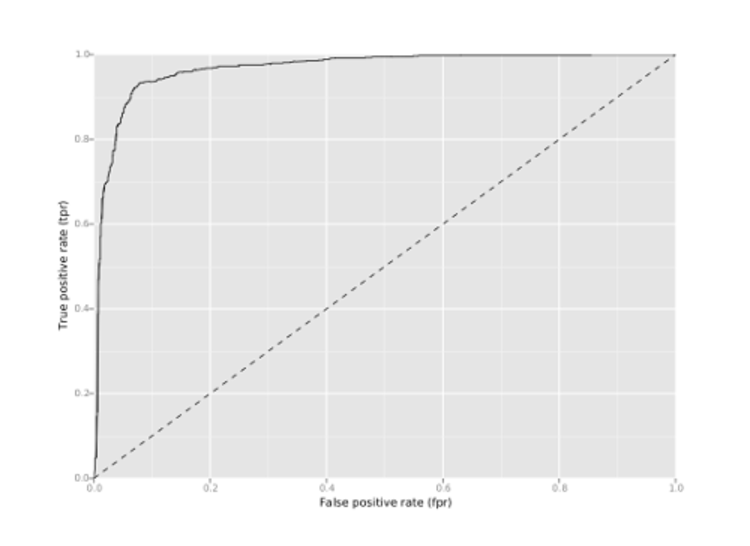
\includegraphics{exp2_roc.pdf}
		\caption{A receiver operating curve (ROC) with 310 thresholds for a trained, linear SVM using the model parameter, C = 0.6. The training data were derived from the "Spambase" dataset.}
	\end{center}
\end{figure}

\subsection{Experiment 2}
A linear SVM model was trained on the processed training dataset (\verb|tr_d|) using the C parameter identified as giving the highest accuracy (C = 0.6) from Experiment 1. After training, the weight vector for the SVM model was obtained. The absolute value of each weight was determined and the 57 features in the \verb|tr_d| dataset were then ranked by their absolute weight from greatest value to least value. A series of SVM models was used to evaluate the test dataset (\verb|te_d|) where, for each evaluation, the highest ranked m features (m = 1, 2, ..., 57) were selected for the SVM model and all other features were set to zero. Thus, the SVM model for the first evaluation of the test dataset used only the highest ranking feature (Feature 26; abs.wgt = 2.4654) with the values for all other features in \verb|te_d| set to zero. This SVM model gave an accuracy of 0.6098. The SVM model for the second evaluation of the test dataset used only the first and second highest ranking features (Feature 26; abs.wgt = 2.4654 and Feature 24; abs.wgt = 1.4083) with the values for all other features in \verb|te_d| set to zero. This second SVM model gave an accuracy of 0.7339. The experimental results for all SVM models are given in Table 3 and are displayed graphically in Figure 2.  The realization of Experiment 2 is documented in the files, \verb|Exp2_FeatureSelection1.py| and \verb|Exp2_FeatureSelection2.py|.

\begin{figure}
	\begin{center}
		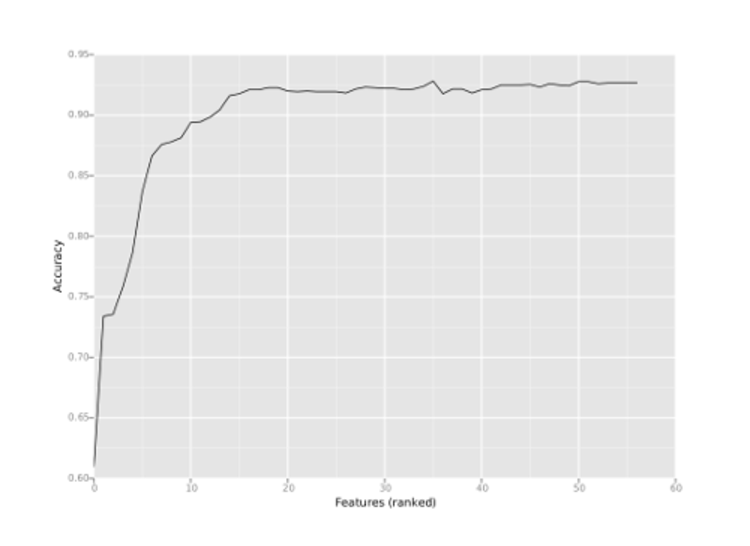
\includegraphics{exp2_accuracies.pdf}
		\caption{The cumulative effect of adding weight-ranked features on the accuracy of the SVM in Experiment 2.}
	\end{center}
\end{figure}

\begin{longtable}[!htbp]{lccc}
\caption{The 57 features used for the SVM in Experiment 2 ranked by the absolute value of their weight and the cumulative effect on the SVM accuracy.} \\
[-1.8ex]\hline \hline \\[-1.8ex] 
 {Rank Order} & {Feature Number} & {SVM weight} & {Cumulative Accuracy} \\
\hline \\[-1.8ex]
\endfirsthead

{\centering {\tablename\ \thetable{} -- continued from previous page}} \\
[1.8ex]\hline \hline \\[-1.8ex] 
{Rank Order} & {Feature Number} & {SVM weight} & {Cumulative Accuracy} \\
\hline \\[-1.8ex]
\endhead

\multicolumn{4}{r}{{Continued on next page ...}} 
\endfoot

\hline 
\endlastfoot

1 & 26 & 2.4654 & 0.6098\\
2 & 24 & 1.4083 & 0.7339\\
3 & 30 & 1.4016 & 0.7356\\
4 & 52 & 1.1448 & 0.7582\\
5 & 45 & 0.9517 & 0.7864\\
6 & 6 & 0.8817 & 0.8366\\
7 & 15 & 0.8394 & 0.8664\\
8 & 44 & 0.7067 & 0.8758\\
9 & 25 & 0.6905 & 0.8780\\
10 & 40 & 0.6637 & 0.8813\\
11 & 41 & 0.6196 & 0.8940\\
12 & 34 & 0.5762 & 0.8945\\
13 & 4 & 0.4973 & 0.8984\\
14 & 23 & 0.4647 & 0.9045\\
15 & 55 & 0.3969 & 0.9161\\
16 & 22 & 0.3652 & 0.9177\\
17 & 53 & 0.3602 & 0.9210\\
18 & 38 & 0.3255 & 0.9210\\
19 & 3 & 0.3071 & 0.9227\\
20 & 28 & 0.2972 & 0.9227\\
21 & 16 & 0.2909 & 0.9199\\
22 & 7 & 0.2876 & 0.9194\\
23 & 43 & 0.2698 & 0.9199\\
24 & 54 & 0.2591 & 0.9194\\
25 & 14 & 0.2567 & 0.9194\\
26 & 32 & 0.2440 & 0.9194\\
27 & 51 & 0.2286 & 0.9183\\
28 & 56 & 0.2272 & 0.9216\\
29 & 29 & 0.2243 & 0.9232\\
30 & 20 & 0.2226 & 0.9227\\
31 & 21 & 0.2024 & 0.9221\\
32 & 27 & 0.1986 & 0.9221\\
33 & 31 & 0.1856 & 0.9210\\
34 & 18 & 0.1719 & 0.9216\\
35 & 48 & 0.1593 & 0.9238\\
36 & 8 & 0.1498 & 0.9282\\
37 & 2 & 0.1333 & 0.9177\\
38 & 10 & 0.1115 & 0.9216\\
39 & 47 & 0.1035 & 0.9216\\
40 & 17 & 0.1033 & 0.9183\\
41 & 9 & 0.0931 & 0.9210\\
42 & 19 & 0.0911 & 0.9216\\
43 & 0 & 0.0907 & 0.9249\\
44 & 39 & 0.0849 & 0.9249\\
45 & 33 & 0.0706 & 0.9249\\
46 & 42 & 0.0680 & 0.9254\\
47 & 46 & 0.0558 & 0.9232\\
48 & 5 & 0.0471 & 0.9260\\
49 & 37 & 0.0354 & 0.9249\\
50 & 11 & 0.0301 & 0.9243\\
51 & 13 & 0.0236 & 0.9277\\
52 & 12 & 0.0234 & 0.9277\\
53 & 35 & 0.0206 & 0.9260\\
54 & 36 & 0.0187 & 0.9266\\
55 & 49 & 0.0014 & 0.9266\\
56 & 1 & 0.0003 & 0.9266\\
57 & 50 & 0.00003 & 0.9266\\
\end{longtable}

\subsection{Experiment 3}
Experiment 3 had exactly the same design as Experiment 2 except that features were ranked randomly rather than being ranked by the absolute value of their weight. The experimental results for all SVM models in Experiment 3 are given in Table 4 and are displayed graphically in Figure 3.  The realization of Experiment 3 is documented in the files, \verb|Exp3_FeatureSelection1.py| and \verb|Exp3_FeatureSelection2.py|.

\begin{figure}
	\begin{center}
		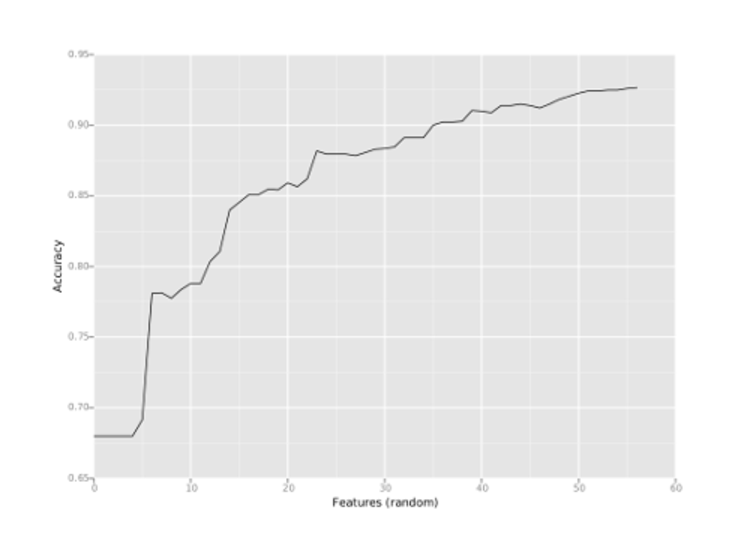
\includegraphics{exp3_accuracies.pdf}
		\caption{The cumulative effect of adding randomly ranked features on the accuracy of the SVM in Experiment 3. }
	\end{center}
\end{figure}

\begin{longtable}[!htbp]{lccc}
\caption{The 57 features used for the SVM in Experiment 2 ranked in random order and the cumulative effect on the SVM accuracy.} \\
[-1.8ex]\hline \hline \\[-1.8ex] 
{Rank Order} & {Feature Number} & {SVM weight} & {Cumulative Accuracy} \\
\hline \\[-1.8ex]
\endfirsthead

{\tablename\ \thetable{} -- continued from previous page} \\
[1.8ex]\hline \hline \\[-1.8ex] 
{Rank Order} & {Feature Number} & {SVM weight} & {Cumulative Accuracy} \\
\hline \\[-1.8ex]
\endhead

\multicolumn{4}{r}{{Continued on next page ...}} 
\endfoot

\hline 
\endlastfoot

1 & 6 & 0.8817 & 0.6799\\
2 & 42 & 0.0680 & 0.6799\\
3 & 31 & 0.1856 & 0.6799\\
4 & 38 & 0.3255 & 0.6799\\
5 & 1 & 0.0003 & 0.6799\\
6 & 17 & 0.1033 & 0.6915\\
7 & 23 & 0.4647 & 0.7809\\
8 & 46 & 0.0558 & 0.7814\\
9 & 2 & 0.1333 & 0.7775 \\
10 & 27 & 0.1986 & 0.7836\\
11 & 21 & 0.2024 & 0.7880\\
12 & 44 & 0.7067 & 0.7880\\
13 & 16 & 0.2909 & 0.8035\\
14 & 48 & 0.1593 & 0.8107\\
15 & 52 & 1.1448 & 0.8399\\
16 & 28 & 0.2972 & 0.8454\\
17 & 4 & 0.4973 & 0.8509\\
18 & 0 & 0.0907 & 0.8509\\
19 & 10 & 0.1115 & 0.8548\\
20 & 18 & 0.1719 & 0.8543\\
21 & 55 & 0.3969 & 0.8592\\
22 & 19 & 0.0911 & 0.8565\\
23 & 47 & 0.1035 & 0.8620\\
24 & 51 & 0.2286 & 0.8818\\
25 & 34 & 0.5762 & 0.8796\\
26 & 33 & 0.0706 & 0.8796\\
27 & 3 & 0.3071 & 0.8796\\
28 & 53 & 0.3602 & 0.8785\\
29 & 56 & 0.2272 & 0.8807\\
30 & 40 & 0.6637 & 0.8830\\
31 & 29 & 0.2243 & 0.8835\\
32 & 11 & 0.0301 & 0.8846\\
33 & 22 & 0.3652 & 0.8912\\
34 & 49 & 0.0014 & 0.8912\\
35 & 13 & 0.0236 & 0.8912\\
36 & 24 & 1.4083 & 0.9001\\
37 & 37 & 0.0354 & 0.9023\\
38 & 50 & 0.00003 & 0.9023\\
39 & 45 & 0.9517 & 0.9028\\
40 & 26 & 2.4654 & 0.9105\\
41 & 9 & 0.0931 & 0.9100\\
42 & 32 & 0.2440 & 0.9089\\
43 & 20 & 0.2226 & 0.9139\\
44 & 43 & 0.2698 & 0.9139\\
45 & 25 & 0.6905 & 0.9150\\
46 & 30 & 1.4016 & 0.9139\\
47 & 12 & 0.0234 & 0.9122\\
48 & 5 & 0.0471 & 0.9150\\
49 & 15 & 0.8394 & 0.9183\\
50 & 35 & 0.0206 & 0.9205\\
51 & 8 & 0.1498 & 0.9227\\
52 & 39 & 0.0849 & 0.9243\\
53 & 7 & 0.2876 & 0.9243\\
54 & 14 & 0.2567 & 0.9249\\
55 & 54 & 0.2591 & 0.9249\\
56 & 41 & 0.6196 & 0.9260\\
57 & 36 & 0.0187 & 0.9266\\
\end{longtable}


\subsection{Results and Discussion}
Although the accuracies for all C parameters in Experiment 1 were quite high ($>$0.92), there was a clear performance peak at C=.06. The high quality of the classifier performance is reflected in the ROC curve. Apparently, the SVM software requires a non-zero value for the C parameter.\\

The SVM model in Experiment 3 produced a ranked order of important features for spam detection in the "Spambase" dataset. The top five features for spam detection, given the conditions of Experiment 3, are given in Table 5. Why it is that "George" and "hp" should be included in an email is unclear, but a quick Google search confirms that these two letter sequences were, in fact, ubiquitous in the content of spam circa 2000. One might conjure various explanations for the remaining three descriptors based on legitimacy and greed. Regardless of why such descriptors are used, building SVM classifiers using features selected based on the rank of the absolute value of their weights appears to be useful. In the current case, using just the top 10 ranked features will provide nearly 90\% accuracy.\\
\vspace{5cm}\\
On the other hand, the use of randomly selected features in Experiment 4 seems, as suspected, to provide little efficacy: reaching about the same level of accuracy as in Experiment 3 would require at least 29 features. Notice also that the shape of the curve in Figure 3 lags behind that of Figure 2 in the rate at which increased accuracy is attained. Finally, both Figure 2 and Figure 3 have an asymptotic character suggesting that little gain in accuracy would be expected beyond a threshold number of features.

\begin{table}[!htbp] \centering 
  \caption{The descriptors of the top five features of the "Spambase" dataset, as ranked by the absolute value of their weights.} 
  \label{} 
\begin{tabular}{lcc} 
\\[-1.8ex]\hline 
\hline \\[-1.8ex] 
 {Rank Order} & {Feature} & {Descriptor}\\
\hline \\[-1.8ex]
1 & 26 &  \verb|word_freq_george|\\
2 & 24 &  \verb|word_freq_hp|\\
3 & 30 &  \verb|word_freq_telnet|\\
4 & 52 &  \verb|char_freq_$|\\
5 & 45 &  \verb|word_freq_edu|\\
\hline \\[-1.8ex]
\end{tabular} 
\end{table}

\subsection{Conclusions}
Linear SVMs appear to be highly successful at the task of binary clustering. Clearly, feature selection is one of the keys to successful SVM performance. Finally, there are undoubtedly additional feature sorting algorithms which could presumably be used in conjunction with the 'ranking by absolute weight' algorithm used here to produce highly efficient classifiers.

    

%\renewcommand{\refname}{\normalfont\selectfont\small \textbf{References}} 
%\bibliographystyle{/usr/local/share/texmf/tex/latex/apacite/apacite}
%\bibliography{/home/bmarron//Desktop/BibTex/2016SoE009}

\end{document}
